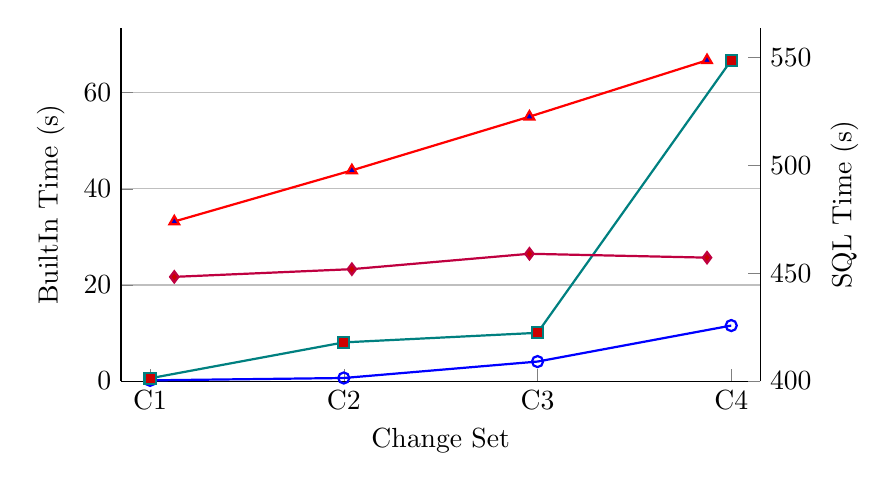
\begin{tikzpicture}
  \begin{axis}[
    name=conflictLeftAxis,
    axis y line*=left,
    axis x line*=bottom,
    ymin=0,
    ymajorgrids,
    xlabel={Change Set},
    ylabel={BuiltIn Time (s)},
    xtick=data,
    symbolic x coords={C1,C2,C3,C4},
    legend to name=collabMergeConflictLegend,
    legend style={draw=none, column sep=1ex, legend columns=2, font=\small},
    width=0.8\linewidth,
    height=0.5\linewidth,
    enlarge x limits=0.05
  ]
    \addplot+[mark=o, thick, color=blue]
      coordinates {(C1,0.15) (C2,0.64) (C3,4.06) (C4,11.55)};
    \addlegendentry{BuiltIn PK Merge}
    \addplot+[mark=square*, thick, color=teal]
      coordinates {(C1,0.58) (C2,8.05) (C3,10.04) (C4,66.74)};
    \addlegendentry{BuiltIn NoPK Merge}
    \addlegendimage{mark=triangle*, thick, color=red}
    \addlegendentry{SQL PK Merge}
    \addlegendimage{mark=diamond*, thick, color=purple}
    \addlegendentry{SQL NoPK Merge}
  \end{axis}

  \begin{axis}[
    axis y line*=right,
    axis x line=none,
    ymin=400,
    ylabel={SQL Time (s)},
    symbolic x coords={C1,C2,C3,C4},
    xtick=data,
    width=0.8\linewidth,
    height=0.5\linewidth
  ]
    \addplot+[mark=triangle*, thick, color=red]
      coordinates {(C1,473.96) (C2,497.65) (C3,522.54) (C4,548.66)};
    \addplot+[mark=diamond*, thick, color=purple]
      coordinates {(C1,448.30) (C2,451.87) (C3,459.00) (C4,457.21)};
  \end{axis}
\end{tikzpicture}

\pgfplotslegendfromname{collabMergeConflictLegend}
